\section{Results}\label{sec:results}

In this paper, we designed a new interpretability technique which can be used to extract knowledge graphs from state clouds of contextual embeddings. We have noticed that NSC is able to successfully recover commonsense relations of abstraction from raw text data (e.g. "apple" IS\_A "fruit", "orange juice" IS\_A "juice", see Fig. \ref{fig:nsc_output_graph}). Additionally, we have found that for a limited number of concepts to relate, the graph search is robust with respect to the starting state. Moreover, the legibility terms included in the linear combination which comprise the search objective (e.g. arc count) successfully nudge the search towards relatively sparse outputs. Finally, the graph search history profile exhibits proper foraging behavior, with fast increases in solution quality in the beginning, followed by a more conservative strategy which ends in marginal improvements towards the move to heavy exploitation (see Fig. \ref{fig:nsc_score_history}).

\begin{figure}[h]
    \centering
    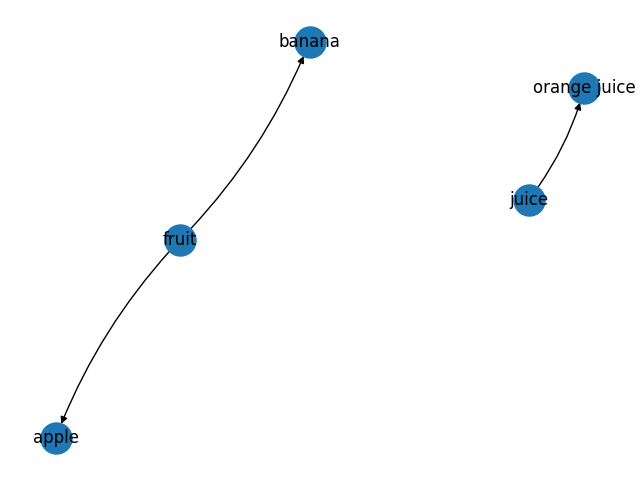
\includegraphics[width=0.45\textwidth]{img/distinct graphs.png}
    \caption{NSC output graph when applied to BERT using several symbols.}\label{fig:nsc_output_graph}
\end{figure}

\begin{figure}[h]
    \centering
    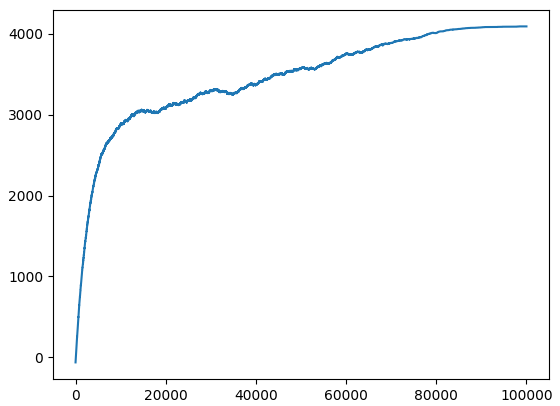
\includegraphics[width=0.45\textwidth]{img/score1.png}
    \caption{Candidate score by epoch during the local graph search.}\label{fig:nsc_score_history}
\end{figure}